\documentclass[xcolor=dvipsnames,notes]{beamer}
\usecolortheme[named=Brown]{structure}
\usetheme{default}
\setbeamertemplate{navigation symbols}{} 
\usepackage{tikz}
\usetikzlibrary{arrows,decorations.pathmorphing,backgrounds,positioning,fit}
\usetikzlibrary{datavisualization.formats.functions}
%     
%Here are some macro's saving time and labour:     
%     
\newcommand{\const}{\mbox{const}}      
\newcommand{\est}{\mbox{{\tiny est}}}      
\newcommand{\im}{\mbox{$\Im \mbox{m}$}}      
\newcommand{\obs}{\mbox{{\tiny obs}}}      
\newcommand{\otherwise}{\mbox{otherwise}}      
\newcommand{\real}{\mbox{$\Re \mbox{e}$}}      
\newcommand{\sign}{\mbox{sign}}      
\newcommand{\sinc}{\mbox{sinc}}      
%
\newcommand{\p}{\mbox{$\partial$}}      
\renewcommand{\d}{\mbox{$\partial$}}      
\newcommand{\w}{\mbox{$\omega$}}      
%
\newcommand{\AAA}{\mbox{\boldmath $A$}}   
\newcommand{\BB}{\mbox{\boldmath $B$}}     
\newcommand{\CC}{\mbox{\boldmath $C$}}     
\newcommand{\DD}{\mbox{\boldmath $D$}}     
\newcommand{\EE}{\mbox{\boldmath $E$}}     
\newcommand{\FF}{\mbox{\boldmath $F$}}   
\newcommand{\GG}{\mbox{\boldmath $G$}}   
\newcommand{\HH}{\mbox{\boldmath $H$}}   
\newcommand{\II}{\mbox{\boldmath $I$}}   
\newcommand{\JJ}{\mbox{\boldmath $J$}}   
\newcommand{\KK}{\mbox{\boldmath $K$}}   
\newcommand{\LL}{\mbox{\boldmath $L$}}   
\newcommand{\MM}{\mbox{\boldmath $M$}}   
\newcommand{\NN}{\mbox{\boldmath $N$}}   
\newcommand{\OO}{\mbox{\boldmath $O$}}   
\newcommand{\PP}{\mbox{\boldmath $P$}}   
\newcommand{\QQ}{\mbox{\boldmath $Q$}}   
\newcommand{\RR}{\mbox{\boldmath $R$}}   
\newcommand{\SSS}{\mbox{\boldmath $S$}}   
\newcommand{\TT}{\mbox{\boldmath $T$}}   
\newcommand{\UU}{\mbox{\boldmath $U$}}   
\newcommand{\VV}{\mbox{\boldmath $V$}}   
\newcommand{\WW}{\mbox{\boldmath $W$}}   
\newcommand{\XX}{\mbox{\boldmath $X$}}   
\newcommand{\YY}{\mbox{\boldmath $Y$}}   
\newcommand{\ZZ}{\mbox{\boldmath $Z$}}   
%
%\newcommand{\aaa}{\mbox{\boldmath $a$}}     
\newcommand{\bb}{\mbox{\boldmath $b$}}     
\newcommand{\cc}{\mbox{\boldmath $c$}}     
\newcommand{\dd}{\mbox{\boldmath $d$}}     
\newcommand{\ee}{\mbox{\boldmath $e$}}   
\newcommand{\ff}{\mbox{\boldmath $f$}}   
%\newcommand{\ggg}{\mbox{\boldmath $g$}}   
\newcommand{\hh}{\mbox{\boldmath $h$}}   
\newcommand{\ii}{\mbox{\boldmath $i$}}   
\newcommand{\jj}{\mbox{\boldmath $j$}}   
\newcommand{\kk}{\mbox{\boldmath $k$}}   
%\newcommand{\lll}{\mbox{\boldmath $l$}}   
\newcommand{\mm}{\mbox{\boldmath $m$}}   
\newcommand{\nn}{\mbox{\boldmath $n$}}   
\newcommand{\pp}{\mbox{\boldmath $p$}}   
\newcommand{\qq}{\mbox{\boldmath $q$}}   
\newcommand{\rr}{\mbox{\boldmath $r$}}   
%\newcommand{\sss}{\mbox{\boldmath $s$}}   
%\newcommand{\ttt}{\mbox{\boldmath $t$}}   
\newcommand{\uu}{\mbox{\boldmath $u$}}   
\newcommand{\vv}{\mbox{\boldmath $v$}}   
\newcommand{\ww}{\mbox{\boldmath $w$}}   
\newcommand{\xx}{\mbox{\boldmath $x$}}   
\newcommand{\yy}{\mbox{\boldmath $y$}}   
\newcommand{\zz}{\mbox{\boldmath $z$}}   
%
\newcommand{\balpha}{\mbox{\boldmath $\alpha$}}     
\newcommand{\bpsi}{\mbox{\boldmath $\psi$}}     
\newcommand{\bphi}{\mbox{\boldmath $\phi$}}     
\newcommand{\bbeta}{\mbox{\boldmath $\beta$}}     
\newcommand{\btheta}{\mbox{\boldmath $\theta$}}     
\newcommand{\bdelta}{\mbox{\boldmath $\delta$}}     
\newcommand{\bgamma}{\mbox{\boldmath $d$}}     
\newcommand{\bGamma}{\mbox{\boldmath $\Gamma$}}     
\newcommand{\bLambda}{\mbox{\boldmath $\Lambda$}}     
\newcommand{\bmu}{\mbox{\boldmath $\mu$}}     
\newcommand{\bnabla}{\mbox{\boldmath $\nabla$}}     
\newcommand{\brho}{\mbox{\boldmath $\rho$}}     
\newcommand{\bSigma}{\mbox{\boldmath $\Sigma$}}     
\newcommand{\bsigma}{\mbox{\boldmath $\sigma$}}     
\newcommand{\bxi}{\mbox{\boldmath $\xi$}}     
\newcommand{\bepsilon}{\mbox{\boldmath $\epsilon$}}     
\newcommand{\blambda}{\mbox{\boldmath $\lambda$}}     
\newcommand{\BLambda}{\mbox{\boldmath $\Lambda$}}     
%-------------------------------------%
%  \Appendix - a new appendix command %
%-------------------------------------%
%The appendix command is used as in
% \Appendix{A}{The wave equation as a matrix equation}
\newcommand {\Appendix}[1]{
              \section*{APPENDIX #1}
              \setcounter{equation}{0}
              \renewcommand{\theequation} 
              {A-\arabic{equation}}}
\newcommand {\Appendices}[2]{
              \section*{APPENDIX #1: #2 }
              \setcounter{equation}{0}
              \renewcommand{\theequation} 
              {#1-\arabic{equation}}}
%------------------------------------%
%    \aref - a new cite command.     % 
%------------------------------------%
\newcommand{\aref}[2]{\nocite{#1}#2} 
%----------------------------------------
%\eqref -an equation reference command
%----------------------------------------
%\newcommand{\eqref}[1]{(\ref{#1})}
%\newcommand{\eqref}[1]{\ref{#1}}

\usepackage{epsfig}
\usepackage{natbib}
\usepackage{graphicx}
\usepackage{multimedia}
\begin{document}
%\setbeamercolor{titlelike}{fg=gray,bg=white}
%\setbeamercolor{itemize item}{fg=gray,bg=white}
%\setbeamercolor{enumerate item}{fg=gray,bg=white}
%\setbeamercolor{block title}{fg=black,bg=white}
%==============================================
\title{TPG4190 Seismic data acquisition and processing}
\author{B. Arntsen}
\institute[NTNU]{
  NTNU\\
  Department of Geoscience and petroleum \\
  \texttt{borge.arntsen@ntnu.no}
}
\date{Trondheim fall 2024}
\begin{frame}
 \titlepage
\end{frame}
%==============================================
%-----------------------------------------
\begin{frame}{Information}
%-----------------------------------------
\begin{enumerate}
  \item Learning objectives
  \item Schedule
  \item Material
  \item Exercises
  \item Project
  \item Exam
  \item Content
\end{enumerate}
\end{frame}
%-----------------------------------------
\begin{frame}{Learning objectives}
%-----------------------------------------
\begin{itemize}
\item {\bf Know} basic theory and principles of seismic
                 data acquisition
\item {\bf Know} key steps in seismic processing
\item {\bf Know} how to derive and
                 apply basic equations that are used in acquisition 
                 and processing of seismic
                 data.
\item {\bf Know} how to perform simple seismic processing of seismic
                  field data.
\end{itemize}
\end{frame}
%-----------------------------------------
\begin{frame}{Schedule}
%-----------------------------------------
\begin{itemize}
\item {\bf Lecture} Every Tuesday  08:15-10:00 PTS1 room P10)
\item {\bf Lecture} Every Wednesday   09:15-11:00 (PTS1 room P13) 
\item {\bf Exercise}Every Wednesday   12:15-12:00       (PTS1 room P13)
\end{itemize}
\end{frame}
%-----------------------------------------
\begin{frame}{Material}
%-----------------------------------------
\begin{itemize}
\item Lecture slides 1-20
\item Lecture notes (Martin Landr\o )
\end{itemize}
\end{frame}
%-----------------------------------------
\begin{frame}{Exercises}
%-----------------------------------------
\begin{itemize}
\item No obligatory exercises
\item Exercises (and solutions) provided
\end{itemize}
\end{frame}
%-----------------------------------------
\begin{frame}{Project}
%-----------------------------------------
\begin{itemize}
\item Obligatory project
\item Processing of Regional Seismic data set from the Pacific
\item Sherwater Reveal processing software
\item Takes place in in the computerlab room 4, PTS1
\item Deliver report by 15. November
\end{itemize}
\end{frame}
%-----------------------------------------
\begin{frame}{Exam}
%-----------------------------------------
\begin{itemize}
\item School exam
\item No aids allowed
\item Grade A-F
\item Project have to be approved
\end{itemize}
\end{frame}
%-----------------------------------------
\begin{frame}{Content}
%-----------------------------------------
\begin{enumerate}
  \item Acquisition of seismic data
  \item Modeling of seismic data
  \item Preprocessing and Noise
  \item Imaging of seismic data
  \item Multiple removal
  \item Tomography
  \item Full Waveform Inversion
  \item Exam
\end{enumerate}
\end{frame}
%-----------------------------------------
\begin{frame}{Acquisition of seismic data}
%-----------------------------------------
\begin{figure}
  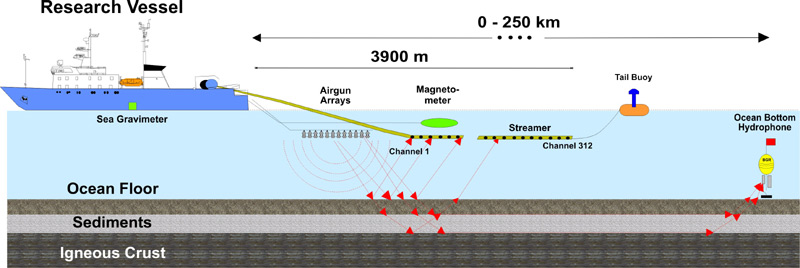
\includegraphics[width=\linewidth]{Fig/seismic-ship.jpg}
  \caption{Seismic ship}
  \label{fig:ship}
\end{figure}
\end{frame}
%-----------------------------------------
\begin{frame}{Modeling of seismic data}
%-----------------------------------------
\begin{figure}
  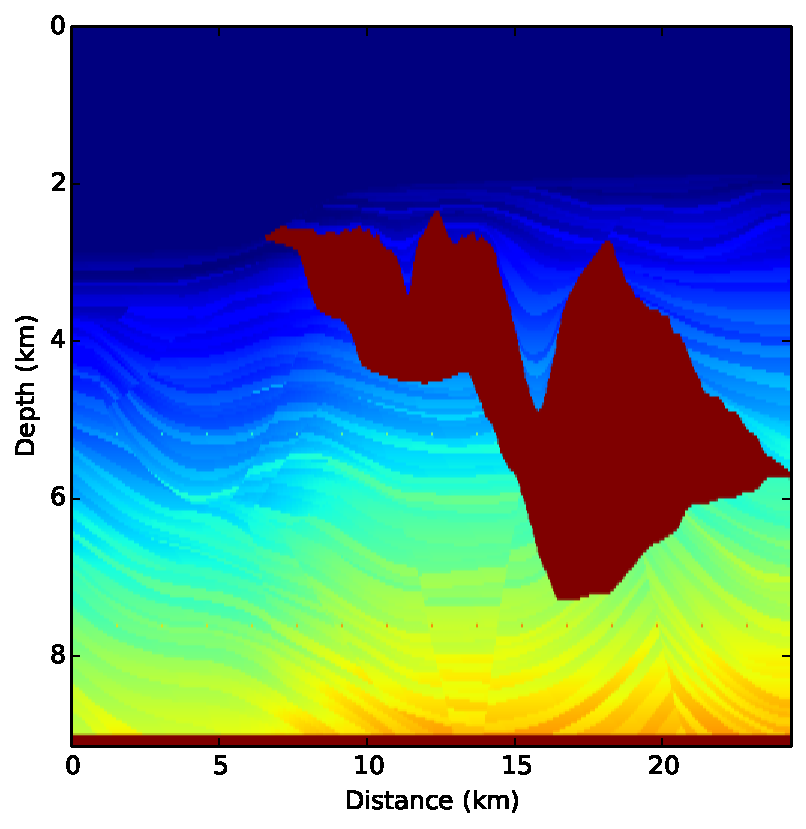
\includegraphics[width=0.4\linewidth]{Fig/vp.pdf}
  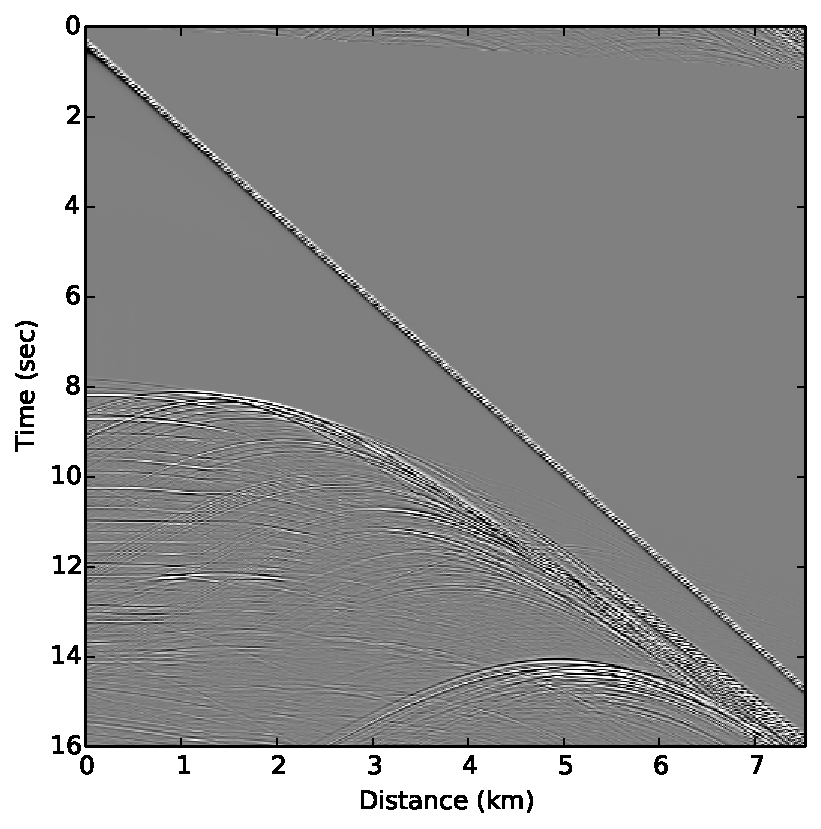
\includegraphics[width=0.4\linewidth]{Fig/data.pdf}
  \caption{Input model (left) and Output data (right)}
\end{figure}
{\bf Movie file:} snp.mp4
%\movie[width=10cm,height=10cm]{Here is the movie}{snp.pdf}
\end{frame}
%-----------------------------------------
\begin{frame}{Preprocessing and Noise}
%-----------------------------------------
\begin{figure}
  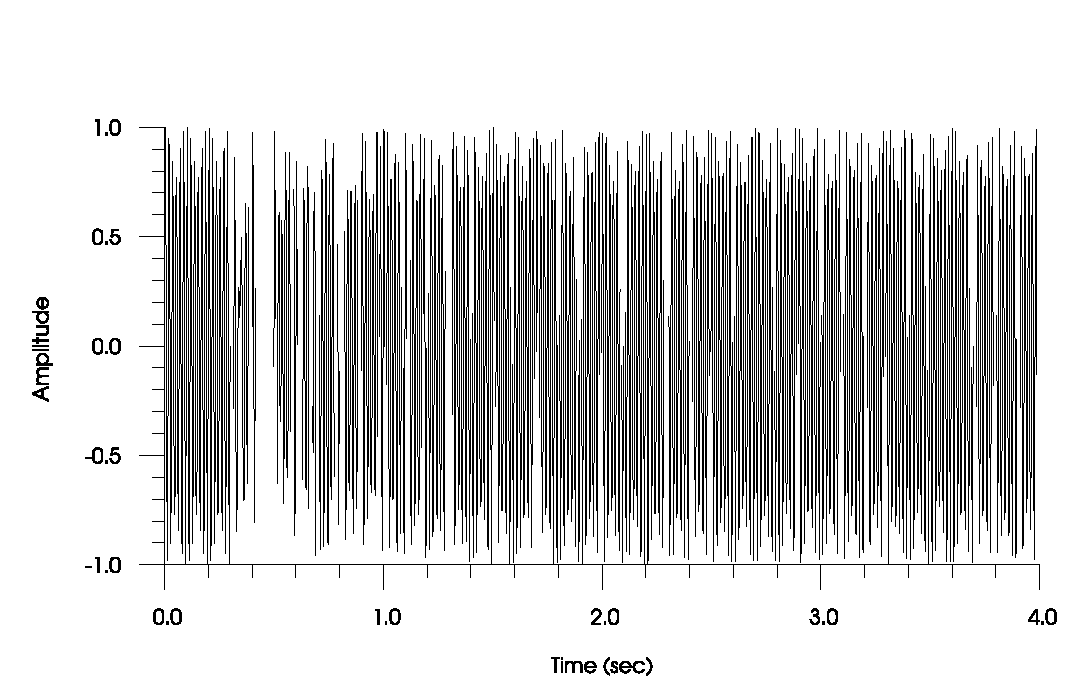
\includegraphics[width=0.5\linewidth]{Fig/ch3-trace.pdf}
  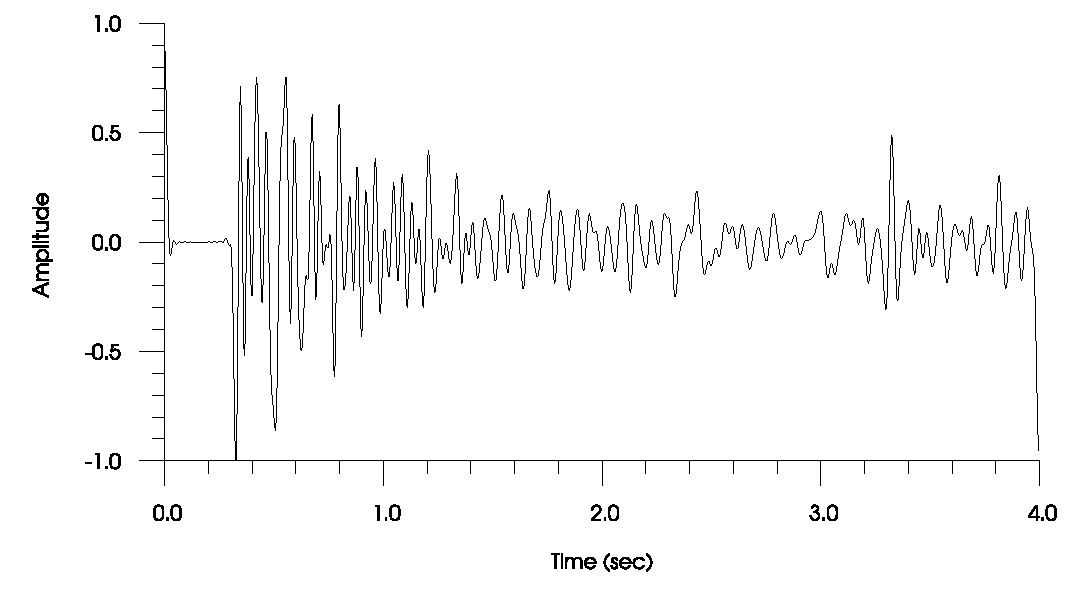
\includegraphics[width=0.5\linewidth]{Fig/ch3-ftrace.pdf}
\end{figure}
\end{frame}
%-----------------------------------------
\begin{frame}{Imaging of Seismic data}
%-----------------------------------------
\begin{figure}
  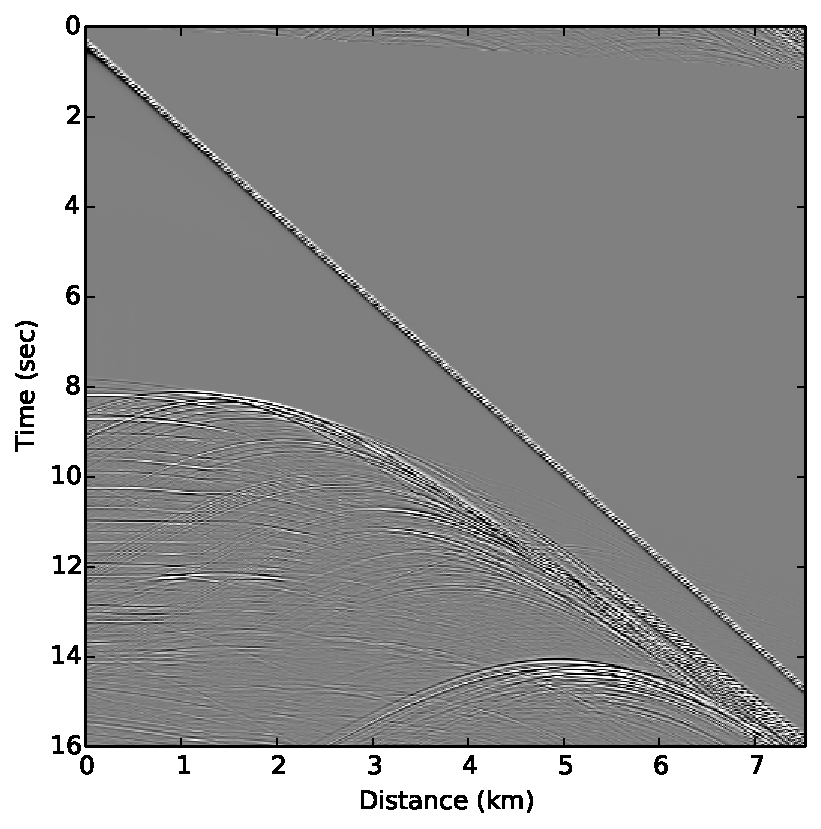
\includegraphics[width=0.4\linewidth]{Fig/data.pdf}
  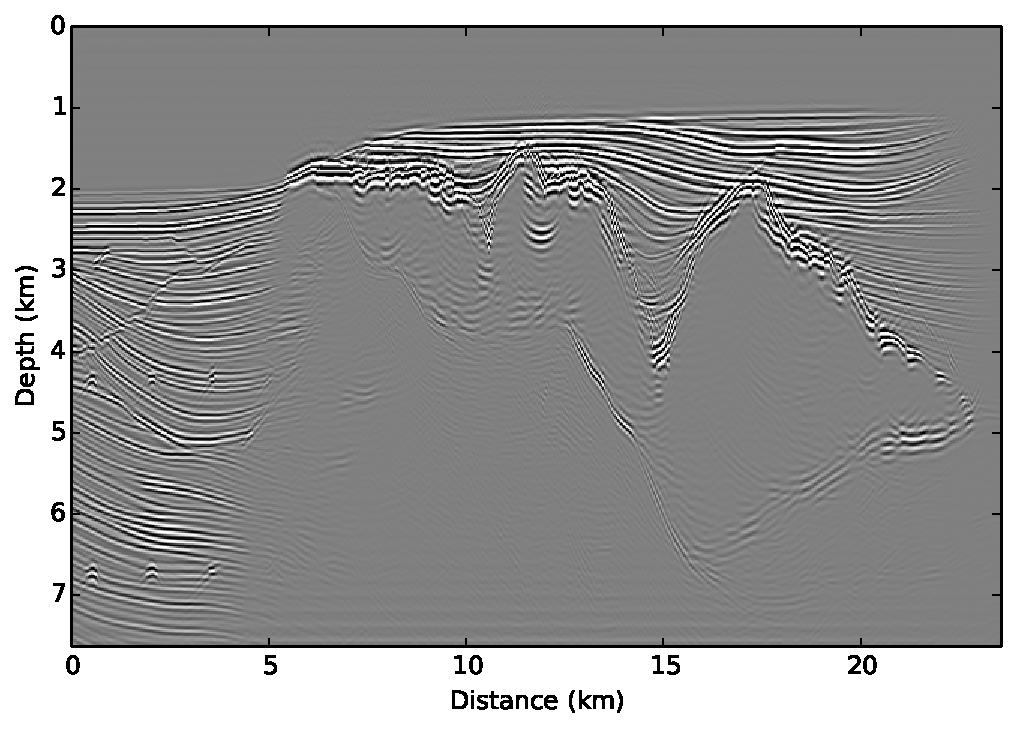
\includegraphics[width=0.4\linewidth]{Fig/mig.pdf}
  \caption{Input data (left) and Output migration (right)}
\end{figure}
\end{frame}
%-----------------------------------------
\begin{frame}{Multiples}
%-----------------------------------------
\begin{figure}
  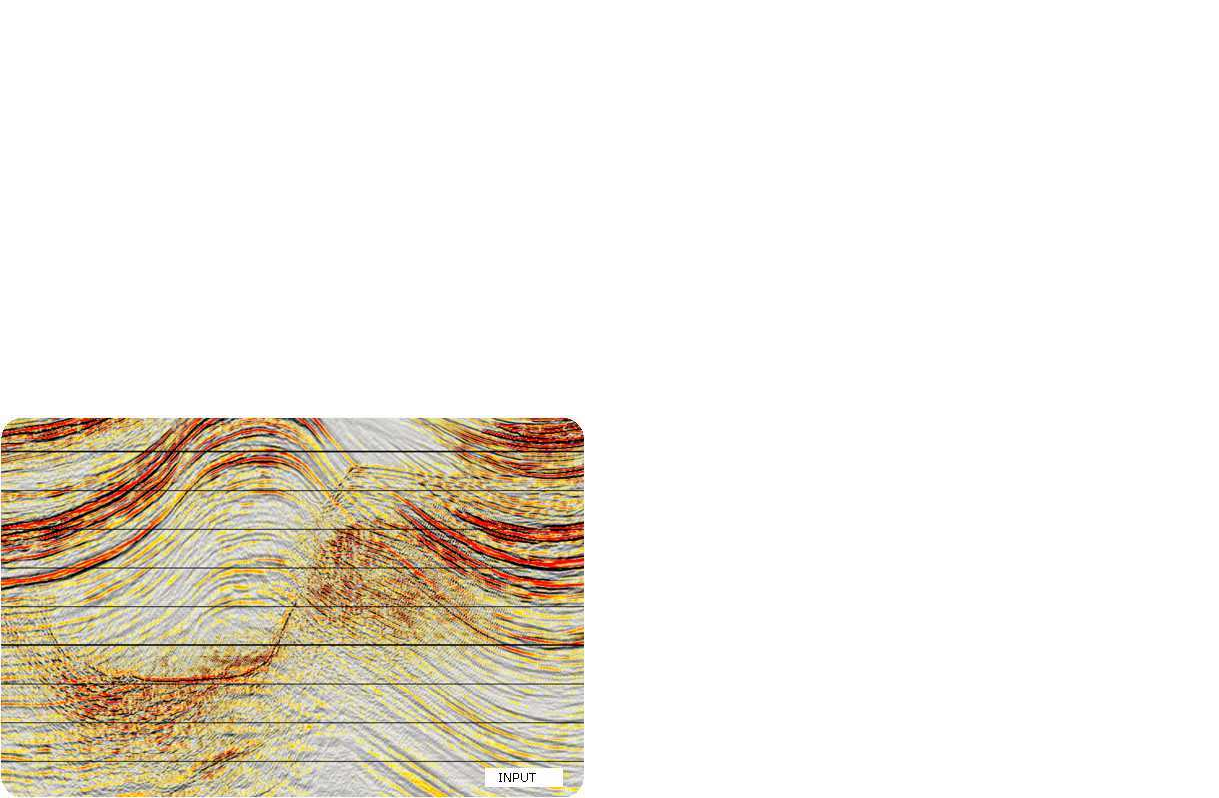
\includegraphics[width=0.5\linewidth]{Fig/ch6-srme1.pdf}
  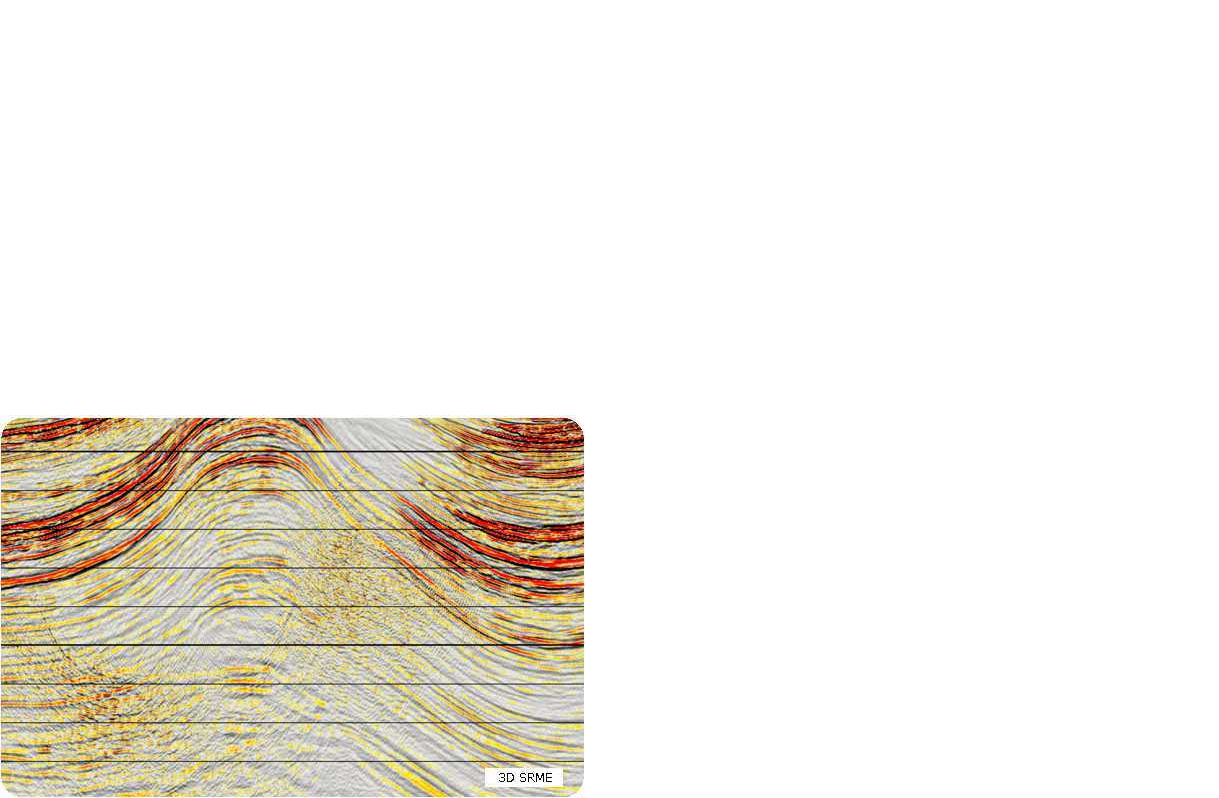
\includegraphics[width=0.5\linewidth]{Fig/ch6-srme2.pdf}
\end{figure}
\end{frame}
%-----------------------------------------
\begin{frame}{Tomography}
%-----------------------------------------
\begin{figure}
  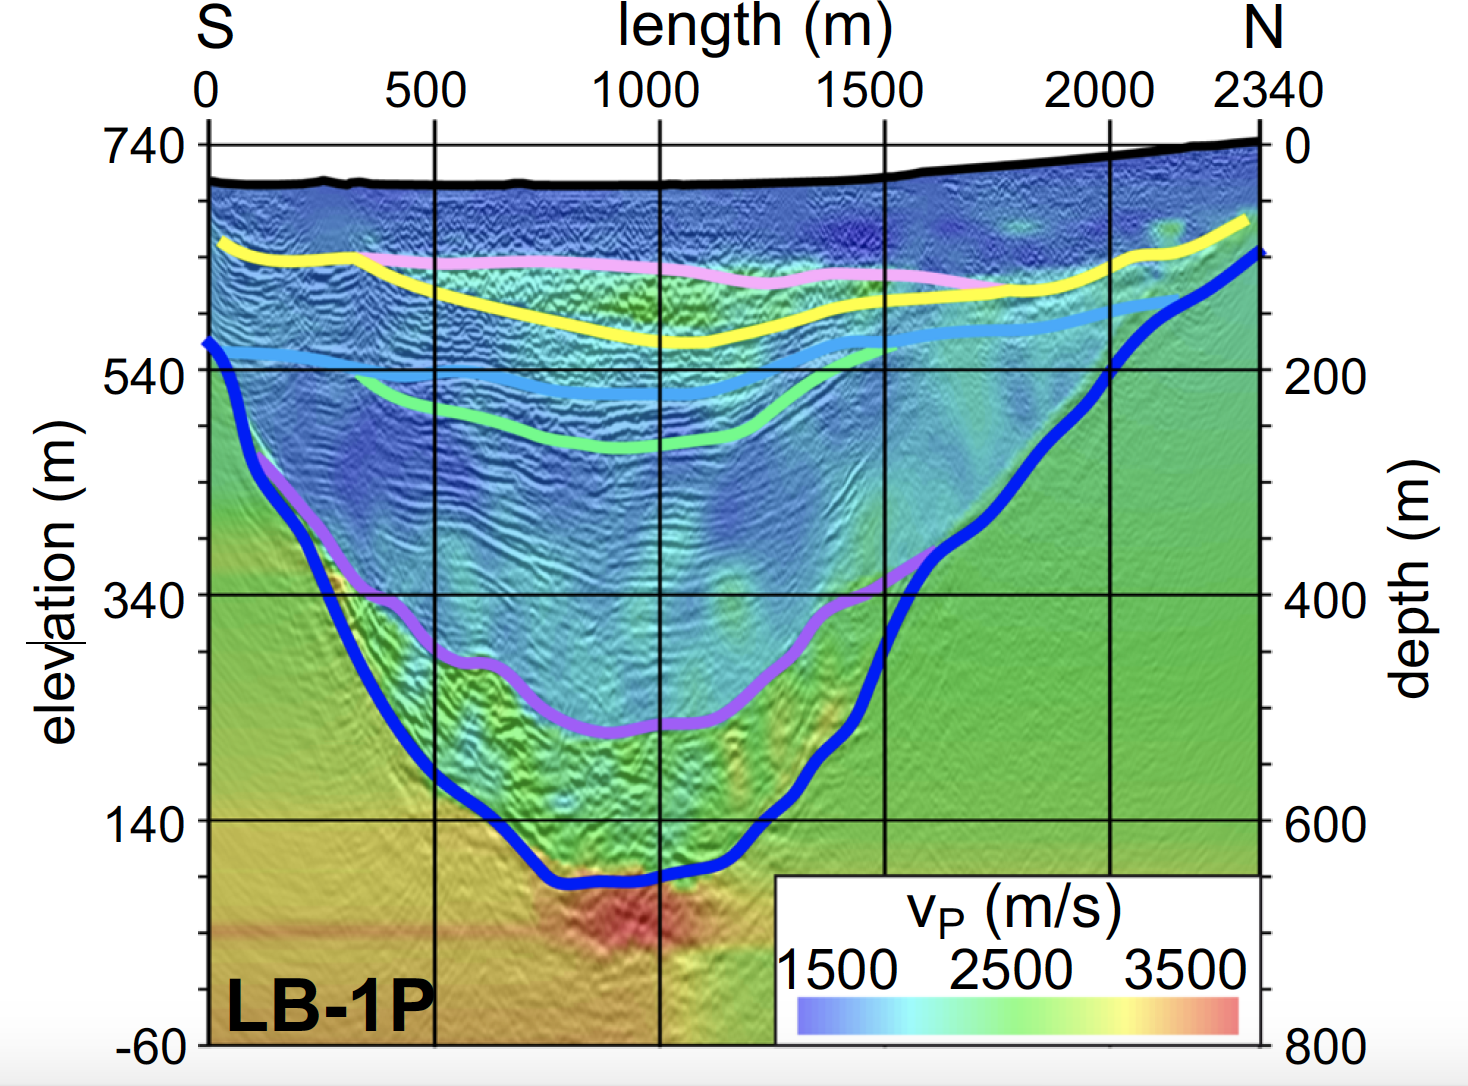
\includegraphics[width=\textwidth]{Fig/tomo.png}
\end{figure}
\end{frame}
%-----------------------------------------
\begin{frame}{Inversion}
%-----------------------------------------
\begin{figure}
  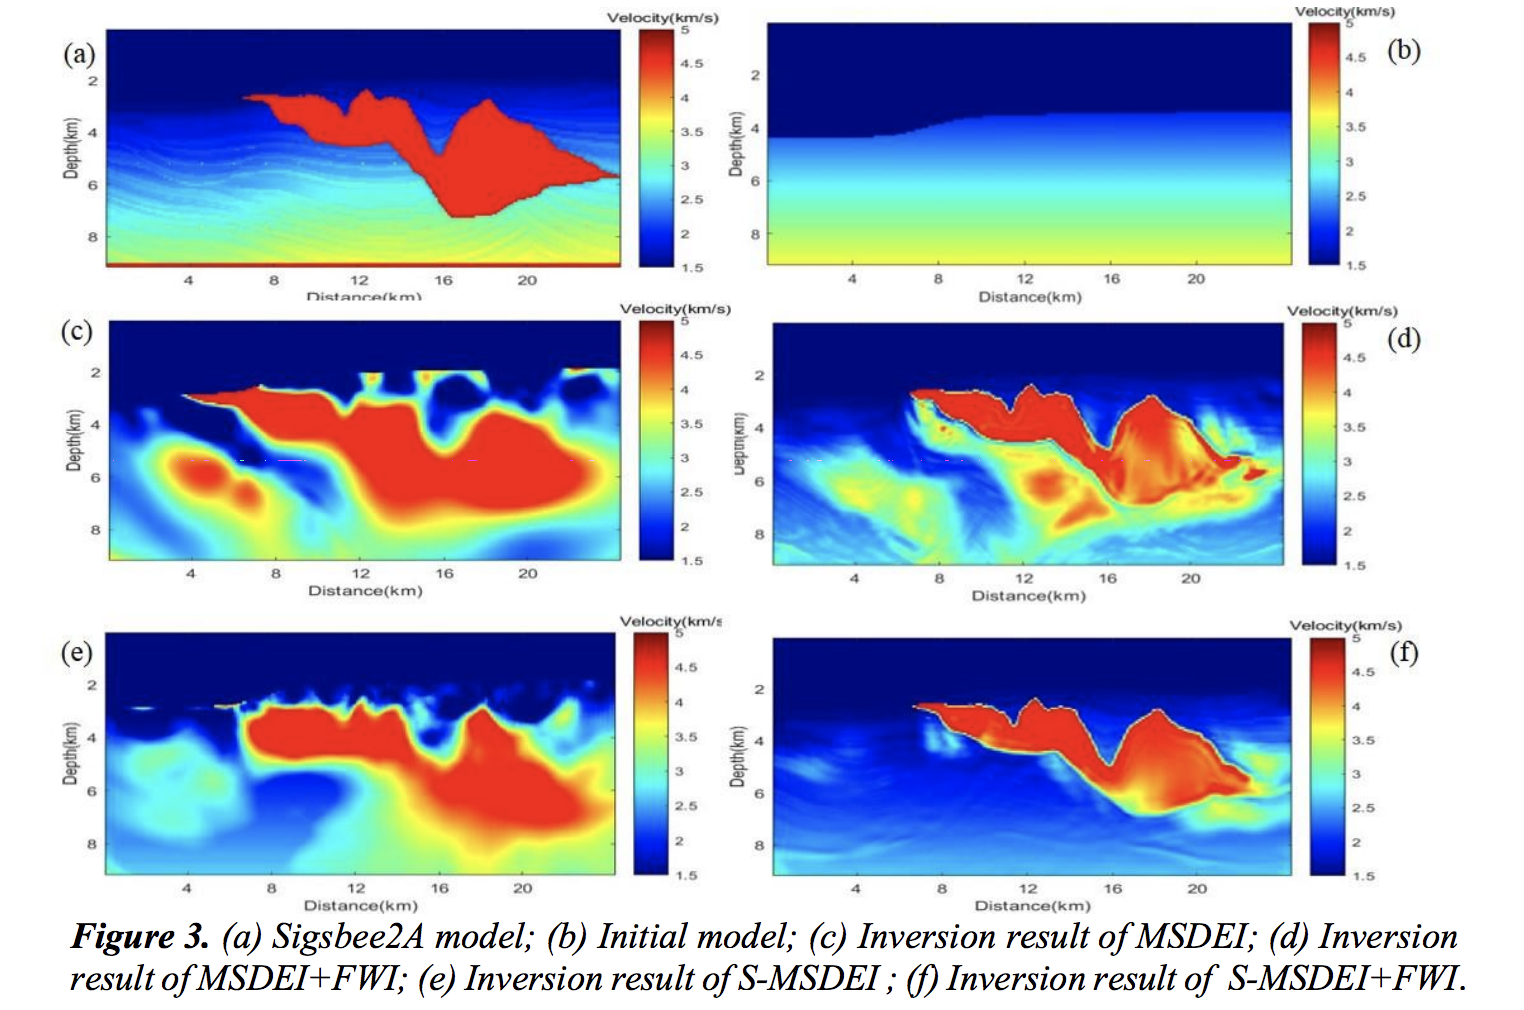
\includegraphics[width=\textwidth]{Fig/fwi.png}
\end{figure}
\end{frame}
\note{ Full waveform inversion of the Sigsbee test model}
%-----------------------------------------
%\begin{frame}{Overview}
%-----------------------------------------
%\end{frame}
\end{document}

